\chapter{Sicurezza degli applicativi}
\section{Integrità del dato}
\subsection{Yup: Validazione frontend e backend}
Per ottenere uno standard qualitativo sui dati inseriti nel database è prevista una stringente e doppia validazione. Infatti sia lato backend che lato frontend è presente una serie di controllo che impediscono inserimenti di dati non conformi alle aspettative. Questa funzionalità è offerta dal package \lstinline[basicstyle=\ttfamily]!Yup!, uno schema builder per il parsing e la validazione di dati.
\subsection{Transazioni SQL}
Nella componente backend è tra le altre cose prevista l'implementazione di transazioni SQL. Una transazione offre la possibilità di creare un punto di ripristino nel caso in cui delle operazioni SQL concatenate non vadano a buon fine. Le transazioni in Garzone sono utilizzate soprattutto in funzioni concernenti pagamenti ed eliminazioni/modifiche/aggiunte a cascata di record, come ad esempio la creazione di un utenza Mailchimp e stripe collegata ad un account di cliente.
\begin{figure}[h!]
    \centering
    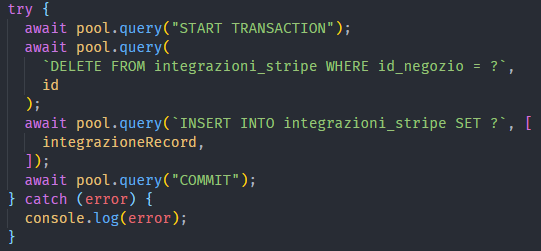
\includegraphics[width=0.8\textwidth]{trans.png}
    \caption{Implementazione in Garzone di una transazione}
\end{figure}
\newpage
\subsubsection{ACID} L'implementazione delle transazioni gode di un insieme di proprietà dette ACID (Atomicity, Consistency, Isolation, Durability)\cite{ACID}. 
\begin{itemize}
    \item \textbf{Atomicità}, la quale prevede che una transazione sia un'unità indivisibile di operazione
    \item \textbf{Consistenza}, la quale prevede che l'esecuzione della  transazione non violi i vincoli di integrità definiti sul database
    \item \textbf{Isolamento}, che prevede che l'esecuzione di una  transazione sia indipendente dall'esecuzione contemporanea di altre  transazioni
    \item \textbf{Persistenza}, che prevede che l'effetto di una transazione che ha eseguito il commit correttamente non venga più perso
\end{itemize}
\section{Sicurezza online}
In Garzone è prevista anche una componente relativa alla sicurezza online, di vitale importanza per evitare che malintenzionati manomettano il corretto funzionamento di tutte le componenti parte dell'applicativo.
\subsection{Whitelist chiamate API}
Una prima protezione riguarda l'interfacciamento dei vari servizi terzi ai vari pannelli. Per ottenere un adeguato livello di protezione è stato previsto che le chiamate verso i servizi Google siano consentite solo dai domini su cui sono presenti i vari pannelli. Un malintenzionato, nel caso in cui dovesse venire in possesso della chiave API che consente le chiamate ai servizi Google, dovrebbe effettuare l'ulteriore operazione di sostituirsi all'host sorgente abilitato alle chiamate. 
\subsection{Firebase Functions Context}
Firebase Authentication mette a disposizione lato backend tra i parametri di una function quello relativo al \lstinline[basicstyle=\ttfamily]!context!, che permette di ottenere e analizzare diversi attributi riguardo la chiamata alla Cloud Function. In Garzone questa funzionalità è servita per validare la corrispondenza tra l'\lstinline[basicstyle=\ttfamily]!uid! (Unique Identifier dell'utente) fornito nei parametri della richiesta e l'\lstinline[basicstyle=\ttfamily]!uid! fornito dal \lstinline[basicstyle=\ttfamily]!context!. In caso i due valori non dovessero coincidere il sistema backend restituisce come risultato un'apposita eccezione \lstinline[basicstyle=\ttfamily]!not-authorized!.
\subsection{Webhook}
Un'altra tecnica per fornire un adeguato livello di sicurezza agli applicativi prevede l'utilizzo di WebHook da parte di servizi esterni per effettuare operazioni sensibili, come il processo di pagamento. Infatti per processare i pagamenti in Garzone è delegata a Stripe la chiamata alla Cloud Function che si occupa di cambiare stato all'ordine. In questo modo è impossibile per un utente malintenzionato effettuare operazioni di cambio stato dell'ordine fingendo un pagamento non effettuato. 
\subsection{Security Rules}
Per quanto riguarda la sicurezza del servizio di Firebase Realtime Database, è stato previsto l'inserimento di regole di sicurezza basati su ciò che un'utenza può ottenere/modificare/eliminare. In Garzone è imposto che ad ogni utenza è possibile accedere solo all'oggetto di Realtime Database che presenta come chiave il proprio \lstinline[basicstyle=\ttfamily]!uid!, ovvero il suo identificativo. Così è impossibile per un'utenza effettuare operazioni malevole su dati relativi ad altre utenze. Le security rules sono state previste anche per il servizio di Cloud Storage prevedendo le stesse caratteristiche imposte sulle utenze riguardo le regole di Realtime Database.